% Written By Enoch Yu
% Downloaded from archive.enochyu.com

\documentclass{article}

\usepackage{amsmath,amsthm,amssymb}
\usepackage{mathtools}

\usepackage{tikz}
\usepackage{tkz-euclide}
\usepackage{hyperref}
\hypersetup{
  colorlinks=true,
  linkcolor=blue,
  filecolor=magenta,      
  urlcolor=cyan,
  pdftitle={2017 PUMaC Geometry A Problem 6},
  pdfpagemode=FullScreen,
}

\usepackage{float}
\usepackage[margin=1in]{geometry}
\usepackage[normalem]{ulem}

\usepackage{fancyhdr}
\pagestyle{fancy}
\fancyhead[R]{Enoch Yu}
\fancyhead[L]{2017 PUMaC Geometry A Problem 6}
\pagenumbering{gobble}

\usepackage{enumitem}
\usepackage{parskip}
\usepackage[dvipsnames]{xcolor}

\newtheorem{theorem}{Theorem}[section]
\newtheorem{lemma}[theorem]{Lemma}
\newtheorem*{lemma*}{Lemma}
\theoremstyle{remark}
\newtheorem*{remark}{Remark}
\newenvironment{solution}{\begin{trivlist}\item[]{\bf Solution}}
    {\qed \end{trivlist}}

\makeatletter
\def\thm@space@setup{%
  \thm@preskip=\parskip \thm@postskip=0pt
}
\makeatother


\title{2017 PUMaC Geometry A Problem 6}
\author{Enoch Yu}
\date{5 October 2025}

\begin{document}
\section*{2017 PUMaC Geometry A Problem 6}
{\color {Gray}
Triangle $ABC$ has $\angle{A} = 90^\circ$, $AB = 2$,
and $AC = 4$. Circle $\omega_1$ has center $C$ and
radius $CA$, while circle $\omega_2$ has center $B$
and radius $BA$. The two circles intersect at point
$E$, different from point $A$. Point $M$ is on
$\omega_2$ and in the interior of $ABC$, such that
$BM$ is parallel to $EC$. Suppose $EM$ intersects
$\omega_1$ at point $K$ and $AM$ intersects $\omega_1$
at point $Z$. What is the area of quadrilateral $ZEBK$?
}

\href{https://youtu.be/ompkS4Li6xo}{Video explanation}
for anyone interested :))

\begin{solution}
Consider the diagram below.

\begin{center}
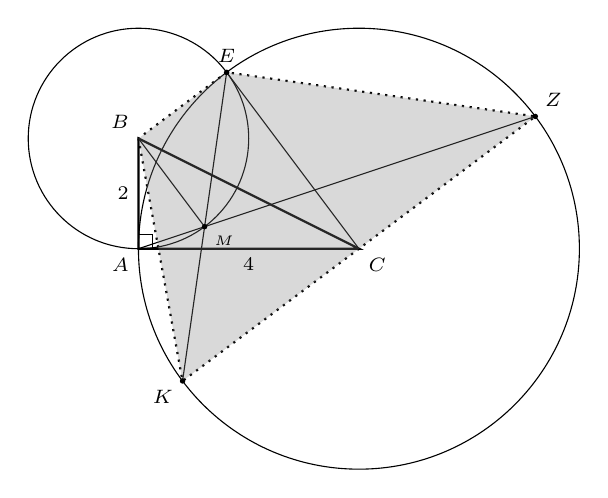
\begin{tikzpicture}[scale=0.7]
    \coordinate (A) at (0,0);
    \coordinate (B) at (0,2);
    \coordinate (C) at (4,0);
    \coordinate (E) at (1.6,3.2);
    \coordinate (M) at (1.2,0.4);
    \coordinate (K) at (0.8,-2.4);
    \coordinate (Z) at (7.2,2.4);

    \draw[thick] (A) -- (B) -- (C) -- cycle;
    \draw (B) circle (2);
    \draw (C) circle (4);

    \draw (B) -- (M);
    \draw (C) -- (E);
    \draw (E) -- (K);
    \draw (A) -- (Z);

    \draw[thick, dotted]
        (B) -- (K) -- (Z) -- (E) -- cycle;
    \fill[gray, opacity=0.3]
        (B) -- (K) -- (Z) -- (E) -- cycle;

    \node at (E)[circle,fill,inner sep=0.7pt]{};
    \node at (M)[circle,fill,inner sep=0.7pt]{};
    \node at (K)[circle,fill,inner sep=0.7pt]{};
    \node at (Z)[circle,fill,inner sep=0.7pt]{};

    \tkzMarkRightAngle[size=.25](B,A,C)

    \node[below left] at (A) {\scriptsize $A$};
    \node[above left] at (B) {\scriptsize $B$};
    \node[below right] at (C) {\scriptsize $C$};
    \node[above] at (E) {\scriptsize $E$};
    \node[below right] at (M) {\tiny $M$};
    \node[below left] at (K) {\scriptsize $K$};
    \node[above right] at (Z) {\scriptsize $Z$};

    \node[left] at ($(A)!0.5!(B)$) {\scriptsize $2$};
    \node[below] at ($(A)!0.5!(C)$) {\scriptsize $4$};
\end{tikzpicture}
\end{center}

First, notice that $\angle{BEC} = 90^\circ$ because
$\triangle{ABC} \cong \triangle{EBC}$ by SSS congruence.
Moreover, $\triangle{BME}$ is an isosceles triangle
with $BM = BE = 2$. Furthermore, since $BM \parallel EC$
by construction, $\angle{BME} = \angle{MEC}$. Therefore,
$\angle{BEM} = \angle{BME} = \angle{MEC} = \angle{MKC}
= 45^\circ$, for $\angle{BEM}  + \angle{MEC} = 90^\circ$.

\begin{center}
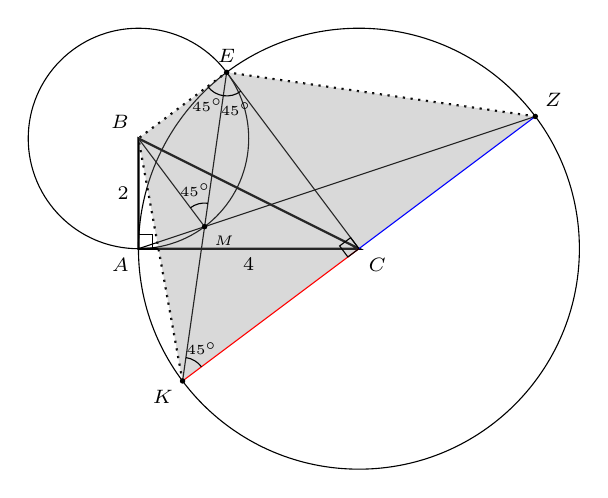
\begin{tikzpicture}[scale=0.7]
    \coordinate (A) at (0,0);
    \coordinate (B) at (0,2);
    \coordinate (C) at (4,0);
    \coordinate (E) at (1.6,3.2);
    \coordinate (M) at (1.2,0.4);
    \coordinate (K) at (0.8,-2.4);
    \coordinate (Z) at (7.2,2.4);

    \draw[thick] (A) -- (B) -- (C) -- cycle;
    \draw (B) circle (2);
    \draw (C) circle (4);

    \draw (B) -- (M);
    \draw (C) -- (E);
    \draw (E) -- (K);
    \draw (A) -- (Z);

    \draw[thick, dotted] (K) -- (B) -- (E) -- (Z);
    \fill[gray, opacity=0.3]
        (B) -- (K) -- (Z) -- (E) -- cycle;
    \draw[red] (K) -- (C);
    \draw[blue] (C) -- (Z);

    \node at (E)[circle,fill,inner sep=0.7pt]{};
    \node at (M)[circle,fill,inner sep=0.7pt]{};
    \node at (K)[circle,fill,inner sep=0.7pt]{};
    \node at (Z)[circle,fill,inner sep=0.7pt]{};

    \tkzMarkRightAngle[size=.25](B,A,C)
    \tkzMarkRightAngle[size=.25](E,C,K)
    \draw pic["\tiny $45^\circ$", draw=black,
        angle radius=0.3cm, angle eccentricity=1.6
    ] {angle=E--M--B};
    \draw pic["\tiny $45^\circ$", draw=black,
        angle radius=0.3cm, angle eccentricity=1.6
    ] {angle=B--E--M};
    \draw pic["\tiny $45^\circ$", draw=black,
        angle radius=0.3cm, angle eccentricity=1.6
    ] {angle=M--E--C};
    \draw pic["\tiny $45^\circ$", draw=black,
        angle radius=0.3cm, angle eccentricity=1.6
    ] {angle=C--K--E};

    \node[below left] at (A) {\scriptsize $A$};
    \node[above left] at (B) {\scriptsize $B$};
    \node[below right] at (C) {\scriptsize $C$};
    \node[above] at (E) {\scriptsize $E$};
    \node[below right] at (M) {\tiny $M$};
    \node[below left] at (K) {\scriptsize $K$};
    \node[above right] at (Z) {\scriptsize $Z$};

    \node[left] at ($(A)!0.5!(B)$) {\scriptsize $2$};
    \node[below] at ($(A)!0.5!(C)$) {\scriptsize $4$};
\end{tikzpicture}
\end{center}

Considering the diagram, if points $K, C, Z$ are
collinear, the area of the quadrilateral $ZEBK$
could be investigated readily.

\begin{lemma*}
Points $K$, $C$, $Z$ are collinear.
\end{lemma*}
\begin{proof}
The fact that $\angle{KCE} = 90^\circ$ was
demonstrated. Therefore, it suffices to show
that $\angle{ECZ} = 90^\circ$.

Notice that $\angle{AZC} = \angle{CAZ}$ and
$\angle{EZA} = \frac{1}{2} \angle{ECA} = \angle{BCA}$.
Therefore, $\angle{EZC} = \angle{BDA}$ from the
diagram below.

\begin{center}
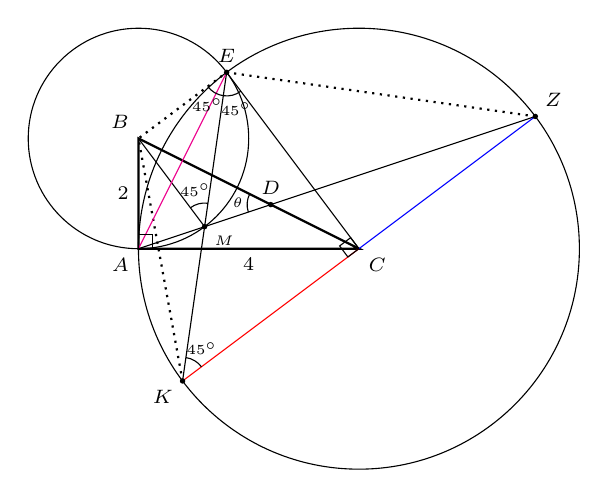
\begin{tikzpicture}[scale=0.7]
    \coordinate (A) at (0,0);
    \coordinate (B) at (0,2);
    \coordinate (C) at (4,0);
    \coordinate (D) at (2.4,0.8);
    \coordinate (E) at (1.6,3.2);
    \coordinate (M) at (1.2,0.4);
    \coordinate (K) at (0.8,-2.4);
    \coordinate (Z) at (7.2,2.4);

    \draw[thick] (A) -- (B) -- (C) -- cycle;
    \draw (B) circle (2);
    \draw (C) circle (4);

    \draw (B) -- (M);
    \draw (C) -- (E);
    \draw (E) -- (K);
    \draw (A) -- (Z);

    \draw[thick, dotted] (K) -- (B) -- (E) -- (Z);
    \draw[red] (K) -- (C);
    \draw[blue] (C) -- (Z);
    \draw[magenta] (A) -- (E);

    \node at (E)[circle,fill,inner sep=0.7pt]{};
    \node at (M)[circle,fill,inner sep=0.7pt]{};
    \node at (K)[circle,fill,inner sep=0.7pt]{};
    \node at (Z)[circle,fill,inner sep=0.7pt]{};
    \node at (D)[circle,fill,inner sep=0.7pt]{};

    \tkzMarkRightAngle[size=.25](B,A,C)
    \tkzMarkRightAngle[size=.25](E,C,K)
    \draw pic["\tiny $45^\circ$", draw=black,
        angle radius=0.3cm, angle eccentricity=1.6
    ] {angle=E--M--B};
    \draw pic["\tiny $45^\circ$", draw=black,
        angle radius=0.3cm, angle eccentricity=1.6
    ] {angle=B--E--M};
    \draw pic["\tiny $45^\circ$", draw=black,
        angle radius=0.3cm, angle eccentricity=1.6
    ] {angle=M--E--C};
    \draw pic["\tiny $45^\circ$", draw=black,
        angle radius=0.3cm, angle eccentricity=1.6
    ] {angle=C--K--E};
    \draw pic["\tiny $\theta$", draw=black,
        angle radius=0.3cm, angle eccentricity=1.4
    ] {angle=B--D--A};

    \node[below left] at (A) {\scriptsize $A$};
    \node[above left] at (B) {\scriptsize $B$};
    \node[below right] at (C) {\scriptsize $C$};
    \node[above] at (D) {\scriptsize $D$};
    \node[above] at (E) {\scriptsize $E$};
    \node[below right] at (M) {\tiny $M$};
    \node[below left] at (K) {\scriptsize $K$};
    \node[above right] at (Z) {\scriptsize $Z$};

    \node[left] at ($(A)!0.5!(B)$) {\scriptsize $2$};
    \node[below] at ($(A)!0.5!(C)$) {\scriptsize $4$};
\end{tikzpicture}
\end{center}
Because $AE$ is the radical axis of $\omega_1$ and
$\omega_2$, $AE \perp BC$.
\[
\angle{EAD} = \frac{1}{2} \angle{EBM} = 45^\circ
\]
Thus, $\theta = 45^\circ = \angle{EZK}$. Because
$\triangle{ECZ}$ is an isosceles triangle,
$\angle{ECZ} = 90^\circ$.
\end{proof}

The proven lemma could be utilized to compute the area.
\begin{align*}
    [BEZK]
    &= [\triangle{BKE}] + [\triangle{EKZ}] \\
    &= \frac{1}{2} \cdot BE \cdot KE \cdot \sin{45^\circ}
        + \frac{1}{2} \cdot KZ \cdot CE \\
    &= \frac{1}{2} \cdot 2 \cdot 4\sqrt{2} \cdot
        \frac{\sqrt{2}}{2} + \frac{1}{2} \cdot 8 \cdot 4 \\
    &= 4 + 16 \\
    &= 20
\end{align*}
Thus, $[BEZK] = 20$.
\end{solution}

\end{document}

